\input templates/header

\usepackage{epigraph}
\usepackage[normalem]{ulem}
\usepackage{xcolor}
\usepackage{colortbl}
\usepackage{tikz}
\usepackage[normalem]{ulem}
\usepackage[absolute,overlay]{textpos}
\usetikzlibrary{trees}
\usetikzlibrary{shapes}
\usetikzlibrary{positioning}

\setlength{\epigraphwidth}{6cm}

\renewcommand*{\arraystretch}{1.2}
\usepackage{xmpmulti}
\usepackage{listings}

\lstset{
  basicstyle=\ttfamily,
  keywordstyle=\color{red}\bfseries,
  commentstyle=\color{blue},
  showstringspaces=false,
  escapeinside={<@}{@>},
}

\newcommand*\circled[1]{\tikz[baseline=(char.base)]{
      \node[circle,ball color=blue, shade, 
 color=white,inner sep=1.2pt] (char) {\tiny #1};}}


\title[ASD - Programmazione Dinamica]{\textbf{Algoritmi e Strutture Dati}\\[24pt]Programmazione dinamica -- Parte 3}

\graphicspath{{figs/13/}}

\begin{document}



%-------------------------------------------------------------------------
\FrameTitle{}

%-------------------------------------------------------------------------
\FrameContent

%%%%%%%%%%%%%%%%%%%%%%%%%%%%%%%%%%%%%%%%%%%%%%%%%%%%%%%%%%%%%%%%%%%%%%%%%%%%%
\section{String matching approssimato}
%%%%%%%%%%%%%%%%%%%%%%%%%%%%%%%%%%%%%%%%%%%%%%%%%%%%%%%%%%%%%%%%%%%%%%%%%%%%%

%-------------------------------------------------------------------------
\begin{frame}{String matching approssimato}

\vspace{-9pt}
\begin{myboxtitle}[Definizione]

Siano:
\BI
\item $P = p_1 \ldots p_m$ una stringa detta \alert{pattern}
\item $T = t_1 \ldots t_n$ una stringa detta \alert{testo}, con $m \leq n$,
\EI

Un'\alert{occorrenza $k$-approssimata} di $P$ in $T$ è una copia di $P$ in $T$ in cui sono ammessi $k$ "errori" tra $P$ e $T$, del seguente tipo:
\begin{enumerate}
\item i corrispondenti caratteri in $P, T$ sono diversi (\alert{sostituzione}) 
\item un carattere in $P$ non è incluso in $T$ (\alert{inserimento})
\item un carattere in $T$ non è incluso in $P$ (\alert{cancellazione})
\end{enumerate}
\end{myboxtitle}

\begin{myboxtitle}[Esempio]
T = \texttt{questoèun\textcolor{red}{o}s\textcolor{red}{c}empio} \\
P = \texttt{~~~~~~~un\textcolor{red}{e}sempio}
\end{myboxtitle}

\end{frame}

%-------------------------------------------------------------------------
\begin{frame}{Esempio}

\vspace{-9pt}
\begin{myboxtitle}[Problema -- Approximated string matching]
Trovare un'occorrenza $k$-approssimata di $P$ in $T$ con $k$ minimo\\ 
($0 \leq k \leq m$).
\end{myboxtitle}

\begin{myboxtitle}[Spiegazione]
\BIL
\item Qual è il minimo valore $k$ per cui si trova un'occorrenza $k$-approssimata di $P$ in $T$?
\item Dove?
\item Con quali errori?
\EIL
\end{myboxtitle}

\end{frame}

%-------------------------------------------------------------------------
\begin{frame}{Sottostruttura ottima}

\vspace{-6pt}
\begin{myboxtitle}[Definizione]
Sia $DP[0 \ldots m][0 \ldots n]$ una tabella di programmazione dinamica
tale che \alert{$DP[i][j]$ sia il minimo valore $k$ per cui esiste un'occorrenza $k$-approssimata di $P(i)$ in $T(j)$ che termina nella posizione $j$}
\end{myboxtitle}

\pause
\BB{Quattro possibilità}
\small
\smallskip
\begin{tabular}{ll}
$DP[i-1][j-1]$, se $P[i] = T[j]$ &	avanza su entrambi i caratteri (uguali) \\
$DP[i-1][j-1]+1$, se $P[i] \neq T[j]$ &	avanza su entrambi i caratteri  (\alert{sost.}) \\
$DP[i-1][j]+1$				& avanza sul pattern (\alert{inserimento})\\
$DP[i][j-1]+1$				& avanza sul testo (\alert{cancellazione})\\
\end{tabular}

\end{frame}

%-------------------------------------------------------------------------
\begin{frame}{Sottostruttura ottima}

\vspace{-6pt}
\[
DP[i][j] = \begin{cases}
0  & \textrm{$i=0$}\\
i  & \textrm{$j=0$}\\
\min\{ DP[i-1][j-1] + \delta, & \delta = \IIF(P[i]=T[j],0,1)\\
\qquad\, DP[i-1][j] + 1,\\ 
\qquad\, DP[i][j-1] + 1\} & \textrm{altrimenti}
\end{cases}
\]

\begin{center}
\IG{0.6}{stringmatching.pdf}
\end{center}

\end{frame}

%-------------------------------------------------------------------------
\begin{frame}{Dove si trova la soluzione finale?}

\vspace{-6pt}
\BIL
\item $DP[m][j] = k$ se e solo se esiste un'occorrenza $k$-approssimata di $P$ in $T(j)$ che
termina nella posizione $j$.
\item La soluzione del problema è data dal più piccolo valore $DP[m][j]$, per $0 \leq j \leq n$
\EIL

\begin{center}
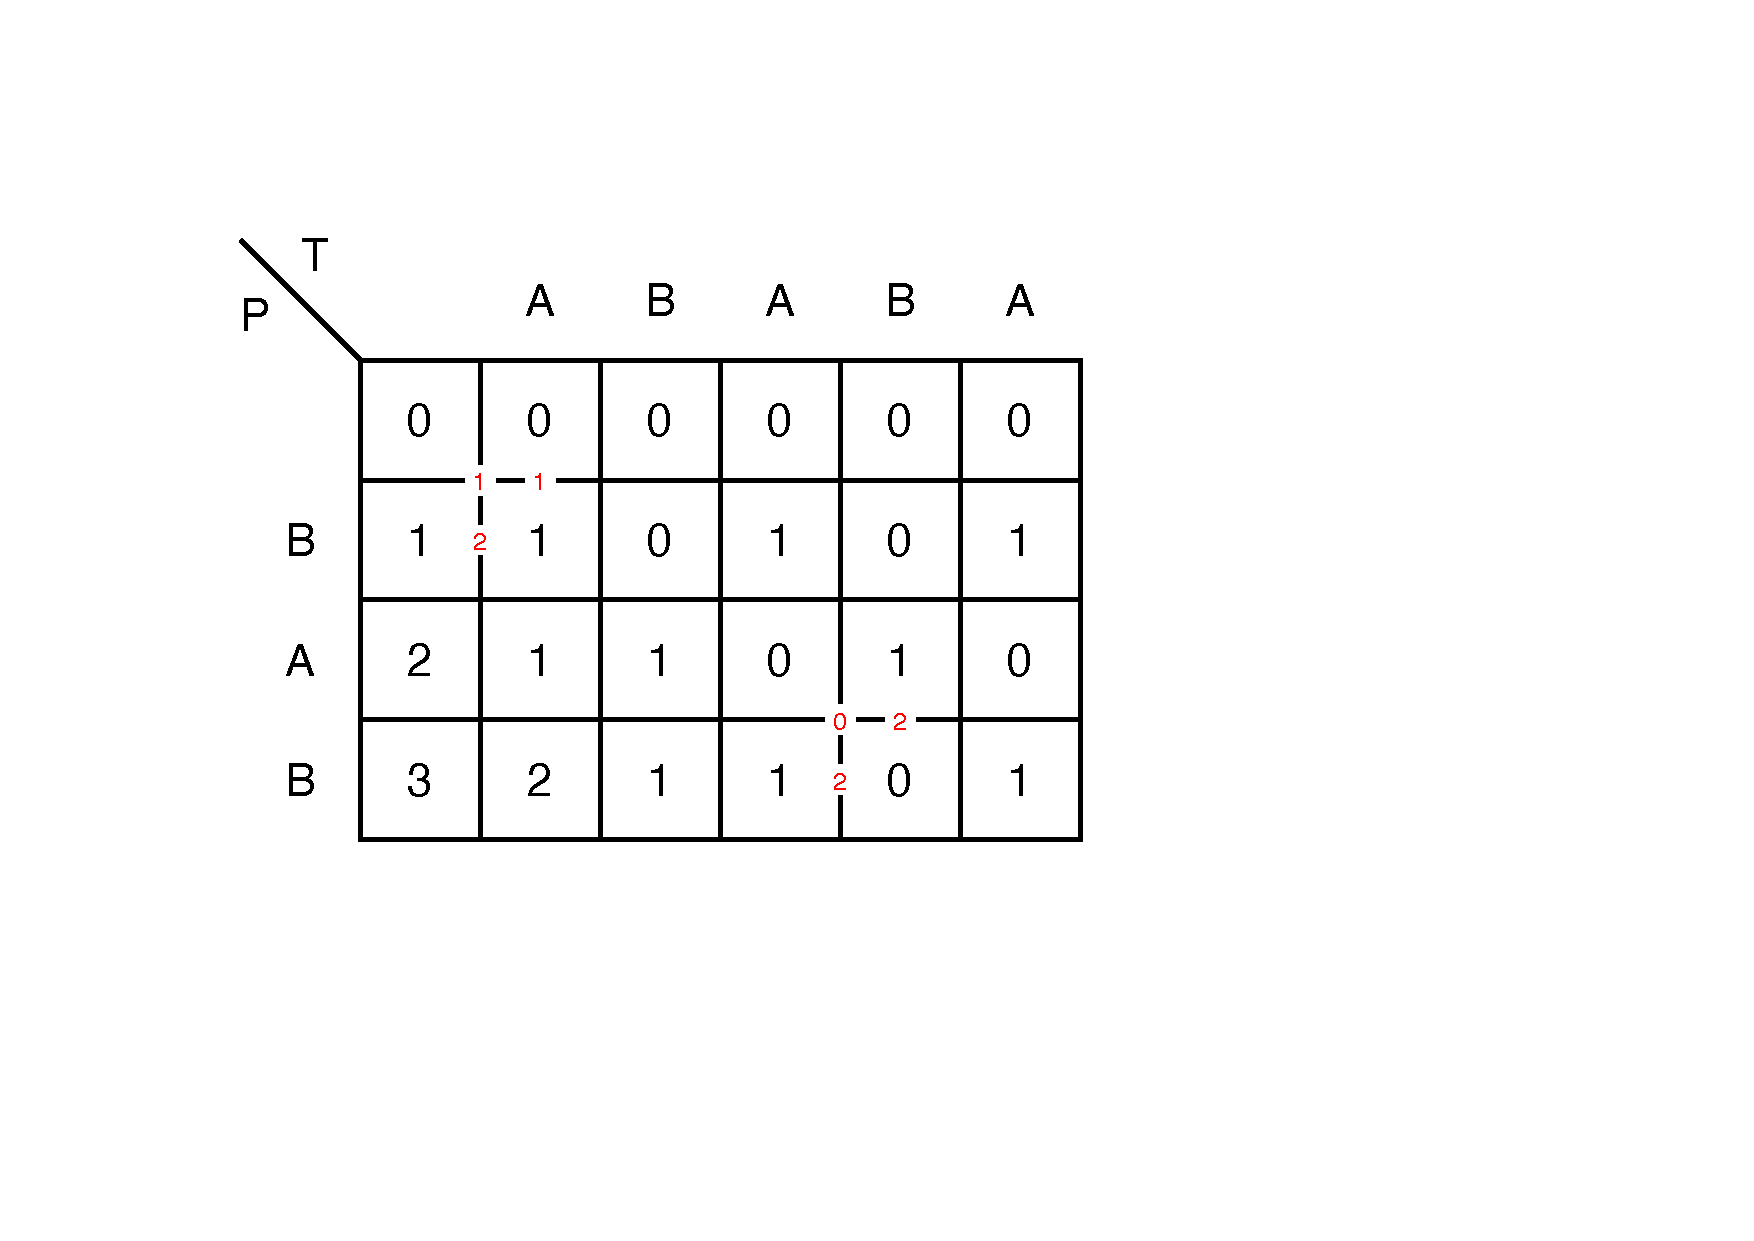
\includegraphics[width=0.5\textwidth]{stringmatching2.pdf}
\end{center}

\end{frame}

%-------------------------------------------------------------------------
\begin{frame}{Algoritmo}

\small
\vspace{-6pt}
\begin{Procedure}
\caption[A]{\INTEGER\ \stringmatching($\Item[\,]\ P,\ \Item[\,]\ T,\ \INTEGER\ m,\ \INTEGER\ n$)}

$\INTARRAY[\,]\ DP = \NEW\ \INTEGER[0 \mldots m][ 0 \mldots n]$\;
\lFor(\Comment*[f]{Caso base: $i=0$}){$j = 0$ \TO\ $n$}{$DP[0][j] = 0$}
\lFor(\Comment*[f]{Caso base: $j=0$}){$i = 1$ \TO\ $m$}{$DP[i][0] = i$}
\For(\Comment*[f]{Caso generale}){$i = 1$ \TO\ $m$}{
  \For{$j = 1$ \TO\ $n$}{
    $DP[i][j] = \MIN(DP[i-1][j-1] + \IIF(P[i] \Eq T[j], 0, 1),$\;
    \qquad\qquad\qquad\ \  $DP[i-1][j]+1,$\;
    \qquad\qquad\qquad\ \  $DP[i][j-1]+1$)\;
  }
}
\INTEGER\ $\Pos = 0$\Comment*{Calcola minimo ultima riga}
\For{$j = 1$ \TO\ $n$}{
  \If{$DP[m][j] < DP[m][\Pos]$}{
    $\Pos = j$\;
  }
}
\Return $\Pos$\;
\end{Procedure}

\end{frame}

%-------------------------------------------------------------------------
\begin{frame}{String matching approssimato}

\vspace{-6pt}
\begin{myboxtitle}[Take-home message -- prendi e porta a casa]
\BIL
\item Non è detto che la  "soluzione finale" si trovi nella casella "in basso a destra"; 
\item \EE invece possibile che la soluzione debba essere ricercata essa 
stessa nella tabella $DP$
\EIL
\end{myboxtitle}

\end{frame}

%-------------------------------------------------------------------------
\begin{frame}{Reality check}

\vspace{-6pt}
\BB{
Approximate String Matching è un esempio di \alert{string metric}:

\begingroup
\small
\begin{quote}
[...] \alert{is a metric that measures distance ("inverse similarity") between two strings} [...]

String metrics are used heavily in information integration and are currently used in areas including fraud detection, fingerprint analysis, plagiarism detection, ontology merging, DNA analysis, RNA analysis, image analysis, evidence-based machine learning, database data deduplication, data mining, incremental search, data integration, and semantic knowledge integration.
\end{quote}
\endgroup

\url{https://en.wikipedia.org/wiki/String_metric}
}

\begin{myboxtitle}[Esempi]
\alert{Edit distance}, detta anche \alert{distanza di Levenshtein}
\end{myboxtitle}

\end{frame}


%%%%%%%%%%%%%%%%%%%%%%%%%%%%%%%%%%%%%%%%%%%%%%%%%%%%%%%%%%%%%%%%%%%%%%%%%%%%%
\section{Prodotto di catena di matrici}
%%%%%%%%%%%%%%%%%%%%%%%%%%%%%%%%%%%%%%%%%%%%%%%%%%%%%%%%%%%%%%%%%%%%%%%%%%%%%


%-------------------------------------------------------------------------
\begin{frame}{Prodotto di catena di matrici}

\vspace{-6pt}
\begin{myboxtitle}[Problema]
Data una sequenza di $n$ matrici $A_1, A_2, A_3, \ldots, A_n$, compatibili due a due al prodotto, vogliamo calcolare il loro prodotto.
\BIL
\item  Il prodotto di matrici non è \alert{commutativo} \ldots .
\item  \ldots .ma è \alert{associativo}: $(A_1 \cdot A_2) \cdot A_3 = A_1 \cdot (A_2 \cdot A_3)$ 
\EIL
\end{myboxtitle}

\begin{myboxtitle}[Cosa vogliamo ottimizzare]
\BIL
\item Il prodotto di matrici si basa sulla \alert{moltiplicazione scalare} come operazione elementare
\item Vogliamo calcolare il prodotto delle $n$ matrici impiegando il più basso numero possibile di moltiplicazioni scalari
\EIL
\end{myboxtitle}

\end{frame}

%-------------------------------------------------------------------------
\begin{frame}{Esempio 1}
    
\vspace{-6pt}
\begin{columns}[T]
\column{0.20\textwidth}
\begingroup
\setlength\arrayrulewidth{1pt}
\begin{tabular}{|c|c|}
\hline
A & $100 \times 1$ \\\hline
B & $1 \times 100$ \\\hline
C & $100 \times 1$ \\\hline
\end{tabular}    
\endgroup
\column{0.75\textwidth}
\vspace{-16pt}    
\IG{1.0}{matrici-esempio1.pdf}
\end{columns}

\end{frame}

%-------------------------------------------------------------------------
\begin{frame}{Esempio 2}

\vspace{-6pt}
\begin{columns}[T]
\column{0.20\textwidth}
\begingroup
\setlength\arrayrulewidth{1pt}
\begin{tabular}{|c|c|}
\hline
A & $50 \times 10$ \\\hline
B & $10 \times 40$ \\\hline
C & $40 \times 30$ \\\hline
D & $30 \times 5$ \\\hline
\end{tabular}    
\endgroup
\column{0.75\textwidth}
\vspace{-16pt}    
\IG{1.0}{matrici-esempio2.pdf}
\end{columns}

\end{frame}


%-------------------------------------------------------------------------
\begin{frame}{Parentesizzazione}

\vspace{-6pt}
\begin{myboxtitle}[Parentesizzazione]
Una \alert{parentesizzazione} $P_{i,j}$ del prodotto $A_i \cdot A_{i+1} \cdot \cdot \cdot A_j$ consiste:
\BI
\item nella matrice $A_i$, se $i = j$; 
\item nel prodotto di due parentesizzazioni ($P_{i,k} \cdot P_{k+1,j}$), altrimenti.
\EI
\end{myboxtitle}

\begin{columns}[T]
\column{0.42\textwidth}
\BB{Esempio}
\[
(A_1 \cdot (A_2 \cdot A_3 ))  \alert{\times}  (A_4 \cdot (A_5 \cdot A_6 )) 
\]
In questo caso, $k=3$ e il prodotto evidenziato 
è detto "\alert{ultimo prodotto}"
\column{0.50\textwidth}
\vspace{-6pt}

\tikzset{
  mynode/.style = {rounded corners,rectangle,draw,fill=yellow!20,minimum width=0.8cm,minimum height=0.8cm}
}

\begin{center}
\begin{tikzpicture}[thick,
  level distance=1.2cm,
  level 1/.style={sibling distance=3.2cm},
  level 2/.style={sibling distance=1.5cm},
  level 3/.style={sibling distance=1.0cm},
  font=\ttfamily\bfseries]
  \node[mynode] {$(A_1 \cdot (A_2 \cdot A_3 ))  \alert{\times}  (A_4 \cdot (A_5 \cdot A_6 ))$}
    child {node[mynode] {$(A_1 \alert{\times} (A_2 \cdot A_3 ))$}
      child {node[mynode] {$A_1$}}
      child {node[mynode] {$(A_2 \alert{\times} A_3 )$}
        child {node[mynode] {$A_2$}}
        child {node[mynode] {$A_3$}}
      }
    }
    child {node[mynode] {$(A_4 \alert{\times} (A_5 \cdot A_6 ))$}
      child {node[mynode] {$A_4$}}
      child {node[mynode] {$(A_5 \alert{\times} A_6 )$}
        child {node[mynode] {$A_5$}}
        child {node[mynode] {$A_6$}}
      }
    };
\end{tikzpicture}
\end{center}

\end{columns}

\end{frame}

%-------------------------------------------------------------------------
\begin{frame}{Parentesizzazione ottima}

\vspace{-6pt}
\begin{myboxtitle}[Parentesizzazione ottima]
La parentesizzazione che richiede il minor numero di moltiplicazioni scalari per essere completata, fra tutte le parentesizzazioni possibili.
\end{myboxtitle}

\begin{myboxtitle}[Motivazione]
Vale la pena preprocessare i dati per cercare la parentesizzazione migliore, per risparmiare tempo dopo nel calcolo vero e proprio
\end{myboxtitle}

\begin{myboxtitle}[Domanda]
Quante sono le parentesizzazioni possibili?
\begin{center}
\begin{tabular}{|c|r|r|r|r|r|r|r|r|r|r|}
\hline
$n$ & \phantom{0}1 & \phantom{0}2 & \phantom{0}3 & \phantom{0}4 & \phantom{0}5 & \phantom{0}6 & \phantom{0}7 & \phantom{0}8 & \phantom{0}9 & \phantom{0}10 \\\hline
$P(n)$ & 1 & 1 & 2 & 5 & ? & ? & ? & ? & ? & ? \\\hline
\end{tabular}
\end{center}
\end{myboxtitle}
\end{frame}

%-------------------------------------------------------------------------
\begin{frame}{Parentesizzazione ottima}

\vspace{-6pt}
\BIL
\item $P(n)$: numero di parentesizzazioni per $n$ matrici $A_1 \cdot \ldots \cdot A_n$
\item L'ultimo prodotto può occorrere in $n-1$ posizioni diverse
\item Fissato l'indice $k$ dell'ultimo prodotto, abbiamo:
\BI
\item $P(k)$ parentesizzazioni per $A_1 \cdot \ldots \cdot A_k$
\item $P(n-k)$ parentesizzazioni per $A_{k+1} \cdot \ldots \cdot A_n$
\EI
\EIL

\[
  P(n) = \begin{cases}
    1 & n = 1 \\
    \sum_{k=1}^{n-1} P(k)P(n-k) & n>1
    \end{cases}
\]

\smallskip
\begin{center}
\begin{tabular}{|c|r|r|r|r|r|r|r|r|r|r|}
\hline
$n$ & \phantom{0}1 & \phantom{0}2 & \phantom{0}3 & \phantom{0}4 & \phantom{0}5 & \phantom{0}6 & \phantom{0}7 & \phantom{0}8 & \phantom{0}9 & \phantom{0}10 \\\hline
$P(n)$ & 1 & 1 & 2 & 5 & 14 & 42 & 132 & 429 & 1430 & 4862 \\\hline
\end{tabular}
\end{center}
\end{frame}

%-------------------------------------------------------------------------
\begin{frame}{Parentesizzazione ottima}

\vspace{-6pt}
\begin{myboxtitle}[Numero di Catalan]
\[
P(n) = C(n) = \frac{1}{n+1} {2n\choose n} = \frac{(2n)!}{(n+1)!n!} = \Theta\left(\frac{4^n}{n \sqrt{n}}\right)
\]
\end{myboxtitle}

\begin{columns}[T]
\column{0.48\textwidth}
\BB{In matematica}
$C(n)$: numero di modi in cui un poligono convesso con $n+2$ lati può essere suddiviso in triangoli.
\IG{0.8}{catalan-hexagon.png}
\column{0.48\textwidth}
\BB{Esercizio}
Dimostrare che $P(n) = \Omega(2^n)$

\BB{Implicazione}
Algoritmi di forza bruta non vanno quindi bene
\end{columns}

\end{frame}

%-------------------------------------------------------------------------
\begin{frame}{Definizioni matematiche}

\begin{tabular}{|P{3cm}|P{8cm}|}
\hline
$A_1 \cdot A_2 \cdot \ldots \cdot A_n$  & il prodotto di $n$ matrici da ottimizzare \\\hline
$c_{i-1}$ & il numero di righe della matrice $A_i$ \\\hline
$c_i$ & il numero di colonne della matrice $A_i$ \\\hline
$A[i \ldots j]$ & il sottoprodotto $A_i \cdot A_{i+1 }\cdot \ldots \cdot A_j$ \\\hline
$P[i \ldots j]$ & una parentesizzazione per $A[i \ldots j]$ \newline(non necessariamente ottima) \\\hline
\end{tabular}
\end{frame}

%-------------------------------------------------------------------------
\begin{frame}{Struttura di una parentesizzazione ottima}
    
\vspace{-6pt}
\begin{myboxtitle}[Osservazioni]
\BIL
\item Sia $A[i \ldots j]$ una sottosequenza del prodotto di matrici
\item Si consideri una parentesizzazione ottima $P[i \ldots j]$ di $A[i \ldots j]$
\item Esiste un \alert{ultimo prodotto}: esiste un indice $k$ tale che 

\[
  P[i\ \ldots j] = P[i \ldots k] \cdot  P[k+1 \ldots j]
\]
\EIL
\end{myboxtitle}

\begin{columns}[T]
\column{0.48\textwidth}
\begin{myboxtitle}[Domanda]
Quali sono le caratteristiche dei due sottoprodotti\\ $P[i \ldots k]$ e $P[k+1 \ldots j]$?
\end{myboxtitle}
\column{0.45\textwidth}
\vspace{-6pt}
\IG{0.8}{sottostruttura.pdf}
\end{columns}

\end{frame}

%-------------------------------------------------------------------------
\begin{frame}{Teorema sottostruttura ottima}

\vspace{-6pt}
\begin{myboxtitle}[Teorema]
\alert{Se} $P[i \ldots j] =  P[i \ldots k]  \cdot P[k+1 \ldots j]$ è una parentesizzazione ottima del prodotto $A[i \ldots j]$, \alert{allora}:
\BI
\item $P[i \ldots k]$ è parentesizzazione ottima del prodotto $A[i \ldots k]$
\item $P[k+1 \ldots j]$ è parentesizzazione ottima del prodotto $A[k+1 \ldots j]$
\EI
\end{myboxtitle}

\begin{myboxtitle}[Dimostrazione -- per assurdo]
\BIL
\item Supponiamo esista un parentesizzazione ottima $P'[i \ldots k]$ di $A[i \ldots k]$ con costo inferiore a $P[i \ldots k]$.
\item Allora, $P'[i \ldots k] \cdot P[k+1 \ldots j]$ sarebbe una parentesizzazione di $A[i \ldots j]$ con costo inferiore a $P[i \ldots j]$, assurdo.
\EIL
\end{myboxtitle}

\end{frame}

% %-------------------------------------------------------------------------
% \begin{frame}{Teorema sottostruttura ottima}
%
% \vspace{-6pt}
% \begin{myboxtitle}[In altre parole]
% Il teorema afferma che esiste una \alert{sottostruttura ottima}: Ogni soluzione ottima al problema della parentesizzazione contiene al suo interno le soluzioni ottime dei due sottoproblemi
% \end{myboxtitle}
%
%
% \begin{myboxtitle}[Programmazione dinamica]
% L'esistenza di sottostrutture ottime ci indica che in questo problema, la programmazione dinamica è applicabile
% \end{myboxtitle}
%
% \begin{myboxtitle}[Prossima fase]
% Definire ricorsivamente il costo di una soluzione ricorsiva
% \end{myboxtitle}
%
%
% \end{frame}

%-------------------------------------------------------------------------
\begin{frame}{Valore della soluzione ottima}

Sia \alert{$DP[i][j]$} il minimo numero di moltiplicazioni scalari necessarie per calcolare il prodotto $A[i \ldots j]$

\BIL
\item \alert{Caso base: $i=j$}. Allora $DP[i][j]=0$
\item \alert{Passo ricorsivo: $i < j$}. Esiste una parentesizzazione ottima 

\[
P[i \ldots j] = P[i \ldots k]  \cdot P[k+1 \ldots j]
\]

Sfruttando la ricorsione:

\[
DP[i][j] = DP[i][k] + DP[k+1][j] + c_{i-1} \cdot c_k \cdot c_j
\]

\item \alert{$c_{i-1} \cdot c_k \cdot c_j$} è il costo per moltiplicare
\BI
\item la matrice $A_i \cdot \ldots A_k$: $c_{i-1}$ righe, $c_k$ colonne
\item la matrice $A_{k+1} \cdot \ldots A_j$: $c_k$ righe, $c_j$ colonne
\EI
\EIL

\end{frame}

%-------------------------------------------------------------------------
\begin{frame}{Valore della soluzione ottima}

\vspace{-6pt}
\IG{0.85}{matrix.pdf}

\end{frame}

%-------------------------------------------------------------------------
\begin{frame}{Valore della soluzione ottima}

\vspace{-6pt}
\BB{Ma qual è il valore di $k$?}
\BIL
\item Non lo conosciamo....
\item ... ma possiamo provarli tutti!
\item $k$ può assumere valori fra $i$ e $j-1$
\EIL

\begin{myboxtitle}[Formula finale]
\small
\[
  DP[i][j] = \begin{cases}
    0 & i=j \\
    \min_{i \leq k < j} \{ DP[i][k] + DP[k+1][j] + c_{i-1} \cdot c_k \cdot c_j \}  & i<j 
  \end{cases}
\]
\end{myboxtitle}

\end{frame}

%-------------------------------------------------------------------------
\begin{frame}{Esempio}
\vspace{-12pt}
\begin{center}
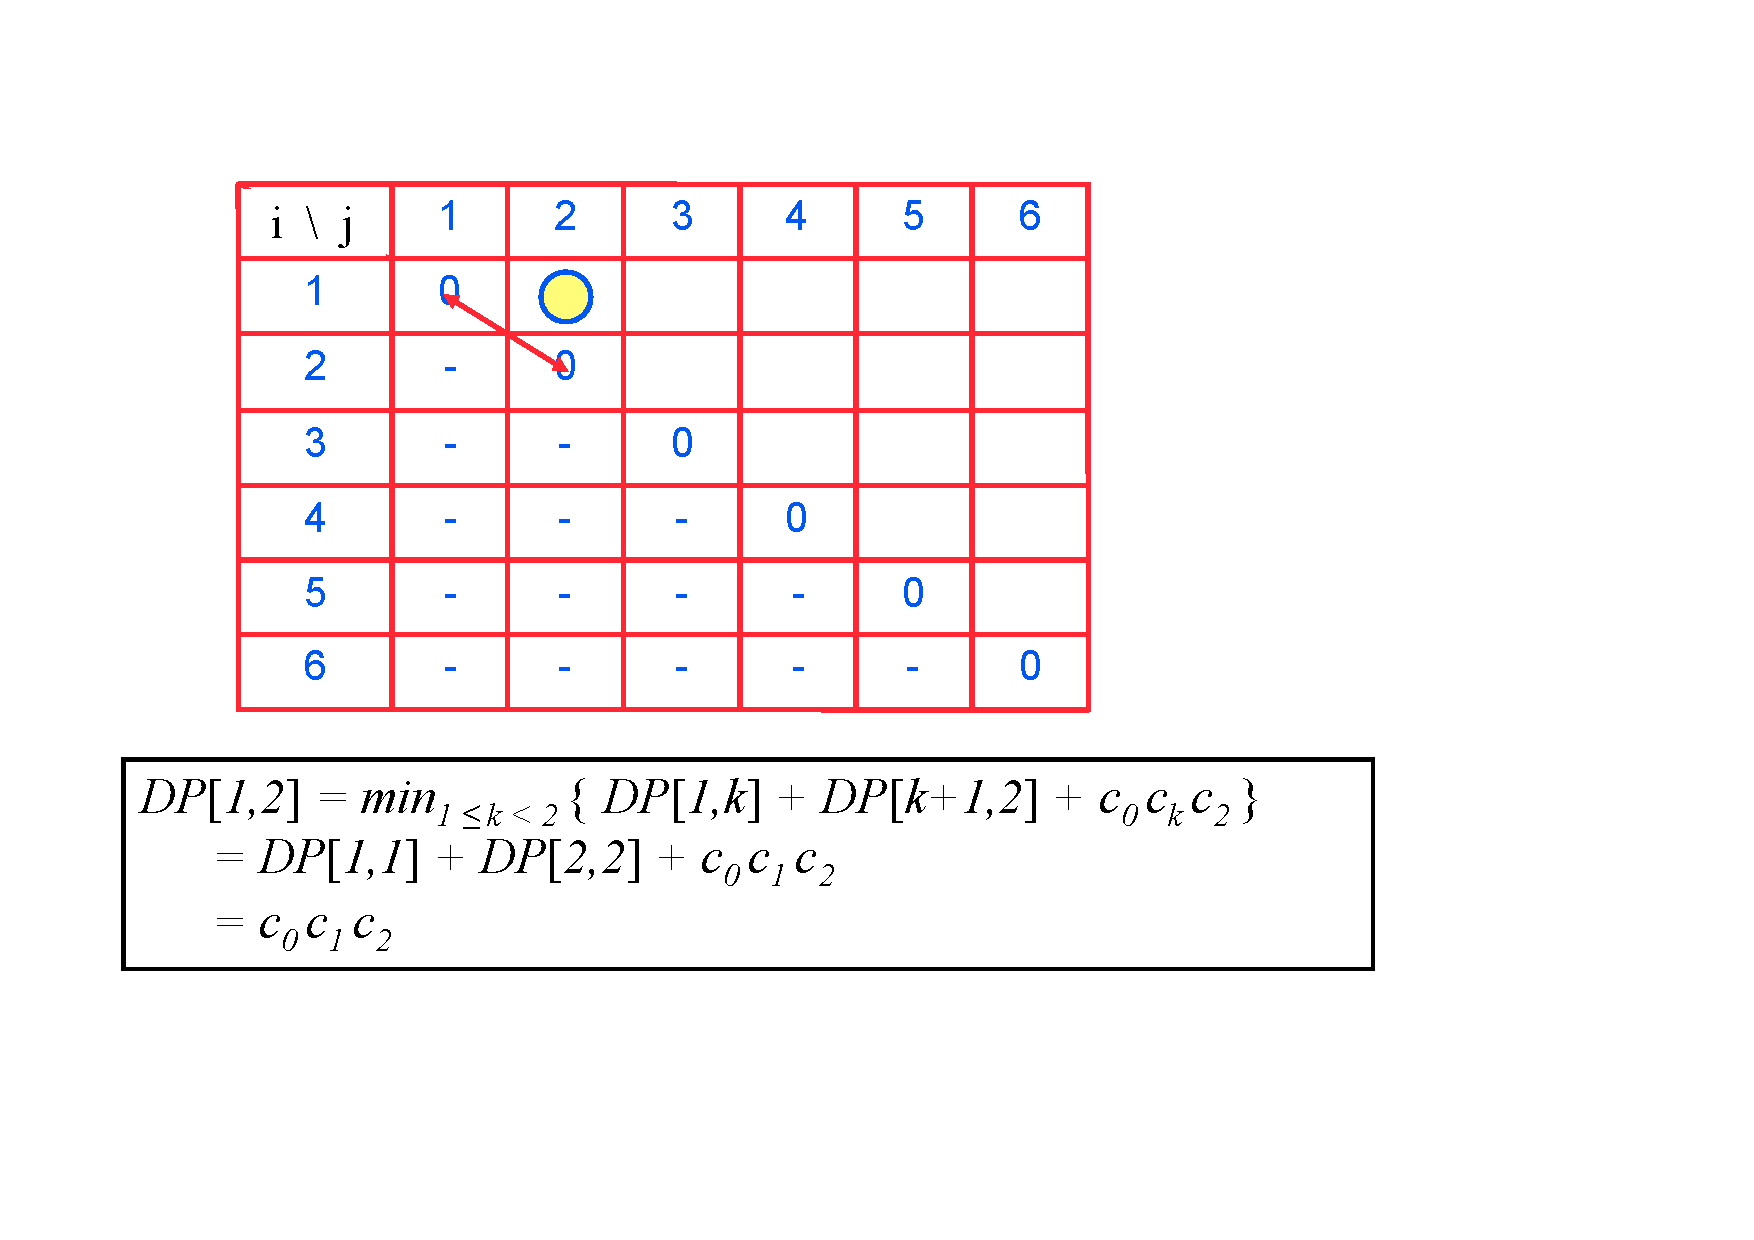
\includegraphics[width=6cm,page=1]{moltmatrici.pdf}
\end{center}
\BB{
\small
\vspace{-13pt}
\begin{align*}
  DP[1][2] &= \min_{1 \leq k < 2} \{ DP[1][k] + DP[k+1][2] + c_0c_kc_2 \} \\
           &= DP[1][1] + DP[2][2] + c_0c_1c_2 \\
           &= c_0c_1c_2
\end{align*}
}

\end{frame}

%-------------------------------------------------------------------------
\begin{frame}{Esempio}
\vspace{-12pt}
\begin{center}
\includegraphics[width=6cm,page=2]{moltmatrici.pdf}
\end{center}
\BB{
\small
\vspace{-13pt}
\begin{align*}
  DP[2][4] &&= \min_{2 \leq k < 4} \{ & DP[2][k] + DP[k+1][4] + c_1c_kc_4 \} \\
           &&= \min  \{ & DP[2][2] + DP[3][4] + c_1c_2c_4, \\
                    && & DP[2][3] + DP[4][4] + c_1c_3c_4 \} 
\end{align*}
}

\end{frame}

%-------------------------------------------------------------------------
\begin{frame}{Esempio}
\vspace{-12pt}
\begin{center}
\includegraphics[width=6cm,page=3]{moltmatrici.pdf}
\end{center}
\BB{
\small
\vspace{-13pt}
\begin{align*}
  DP[2][5] &&= \min_{2 \leq k < 5} \{ & DP[2][k] + DP[k+1][5] + c_1c_kc_5 \} \\
           &&= \min \{ & DP[2][2] + DP[3][5] + c_1c_2c_5, \\
                     && &  DP[2][3] + DP[4][5] + c_1c_3c_5, \\
                     && & DP[2][4] + DP[5][5] + c_1c_4c_5  \} 
\end{align*}
}
\end{frame}

%-------------------------------------------------------------------------
\begin{frame}{Esempio}
\vspace{-12pt}
\begin{center}
\includegraphics[width=6cm,page=4]{moltmatrici.pdf}
\end{center}
\BB{
\small
\vspace{-13pt}
\begin{align*}
  DP[1][5] &&= \min_{1 \leq k < 5} \{ & DP[1][k] + DP[k+1][5] + c_0c_kc_5 \} \\
           &&= \min \{ & DP[1][1] + DP[2][5] + c_0c_1c_5, \\
                    && & DP[1][2] + DP[3][5] + c_0c_2c_5, \\
                    && & DP[1][3] + DP[4][5] + c_0c_3c_5, \\
                    && & DP[1][4] + DP[5][5] + c_0c_4c_5 \} 
\end{align*}
}
\end{frame}

%-------------------------------------------------------------------------
\begin{frame}{Esempio}
\vspace{-12pt}
\begin{center}
\includegraphics[width=6cm,page=5]{moltmatrici.pdf}
\end{center}
\vspace{-3pt}
\BB{
\small
\vspace{-13pt}
\begin{align*}
  DP[1][6] &= \min_{1 \leq k < 6} \{ && DP[1][k] + DP[k+1][6] + c_0c_kc_6 \} \\
           &= \min \{ && DP[1][1] + DP[2][6] + c_0c_1c_6, \\
                   && & DP[1][2] + DP[3][6] + c_0c_2c_6, \\
                   && & DP[1][3] + DP[4][6] + c_0c_3c_6, \\
                   && & DP[1][4] + DP[5][6] + c_0c_4c_6, \\
                   && & DP[1][5] + DP[6][6] + c_0c_5c_6 \} 
\end{align*}
}
\end{frame}

%-------------------------------------------------------------------------
\begin{frame}{Dalla formula al codice}

\vspace{-6pt}
\begin{myboxtitle}[Input]
\BIL
\item Un vettore $c[0 \ldots n]$ contenente le dimensioni delle matrici
\BI
\item $c[0]$ è il numero di righe della prima matrice
\item $c[i-1]$ è il numero di righe della matrice $A_i$
\item $c[i]$ è il numero di colonne della matrice $A_i$
\EI
\item Due indici $i$, $j$ che rappresentano l'intervallo di matrici da moltiplicare
\EIL
\end{myboxtitle}

\begin{myboxtitle}[Output]
Il numero di moltiplicazioni scalari per calcolare il prodotto delle matrici comprese fra gli indici $i$ e $j$
\end{myboxtitle}

\end{frame}

%-------------------------------------------------------------------------
\begin{frame}{Approccio ricorsivo}

\vspace{-6pt}
\begin{Procedure}
\caption[A]{\INTEGER \fontproc{recPar}($\INTEGER[\,]\ c$, \INTEGER $i$, \INTEGER $j$)}
\eIf{$i \Eq j$}
{ \Return\ $0$\; }
{
  $\mathit{minSoFar} = +\infty$\;
  \For{\INTEGER $k = i$ \TO\ $j-1$}{
    \INTEGER $\mathit{val} = \fontproc{recPar}(c, i, k) +  \fontproc{recPar}(c, k+1, j) + c[i-1] \cdot c[k] \cdot c[j]$\;
    \If{$\mathit{val} < \mathit{minSoFar}$}{$\mathit{minSoFar} = \mathit{minSoFar}$\;}
  }
  \Return $\mathit{minSoFar}$\;
}
\end{Procedure}

\BB{Complessità?}

\end{frame}

%-------------------------------------------------------------------------
\begin{frame}{Valutazione}

\vspace{-6pt}
\BB{Alcune riflessioni}
\BIL
\item La soluzione ricorsiva top-down è $\Omega(2^n$)
\item Non è poi migliore dell'approccio basato su forza bruta!
\item Il problema è che molti sottoproblemi vengono risolti più volte
\item Il numero di sottoproblemi è $\frac{n(n+1)}{2}$
\EIL

\end{frame}

%-------------------------------------------------------------------------
\begin{frame}{Versione bottom-up}

\vspace{-6pt}
\begin{myboxtitle}[Tabelle programmazione dinamica]
Due matrici $DP$, $\mathit{last}$ di dimensione $n \times n$ tali che:
\BIL
\item $DP[i][j]$ contiene il numero di moltiplicazioni scalari necessarie
per moltiplicare le matrici $A[i \ldots j]$
\item $\mathit{last}[i][j]$ contiene il valore $k$ dell'ultimo prodotto che minimizza il costo per il sottoproblema
\EIL
\end{myboxtitle}
\end{frame}

%-------------------------------------------------------------------------
\begin{frame}[shrink=10]{Versione bottom-up}

\vspace{-6pt}
\begin{Procedure}
\caption[A]{\textsf{computePar}($\INTARRAY\ c$, \INTEGER $n$)}	
$\INTARRAY[\,]\ DP = \NEW\ \INTEGER[1 \ldots n][1 \ldots n]$\;
$\INTARRAY[\,]\ \mathit{last} = \NEW\ \INTEGER[1 \ldots n][1 \ldots n]$\;
\For(\Comment*[f]{Fill main diagonal}){$i = 1$ \TO $n$}{$DP[i][i] = 0$\;}
\For(\Comment*[f]{$h$: diagonal index}){$h = 2$ \TO $n$}
{
  \For(\Comment*[f]{$i$: row}){$i = 1$ \TO\ $n-h+1$}
  {
    \INTEGER $j = i+h-1$\Comment*{$j$: column}
    $DP[i][j] = +\infty$\;
    \For(\Comment*[f]{$k$: last product}){$k = i$ \TO\ $j-1$} 
    {
      \INTEGER\ $\mathit{temp} = DP[i][k] + DP[k+1][j] + c[i-1] \cdot c[k] \cdot c[j]$\;
      \If{$\mathit{temp} < DP[i][j]$} 
      {
        $DP[i][j] = \mathit{temp}$\;
        $\mathit{last}[i][j] = k$\;
      }
    }
  }
}
\Return $DP[1][n]$\;
\end{Procedure}

\end{frame}


%-------------------------------------------------------------------------
\begin{frame}{}

\begingroup
\renewcommand*{\arraystretch}{1.0}
\vspace{-6pt}
\begin{columns}[T]
\column{0.68\textwidth}
\begin{tabular}{|r|r|r|r|r|r|r|}
\hline
$DP$ &  \textbf{1} & \textbf{2} & \textbf{3} & \textbf{4} & \textbf{5} & \textbf{6} \\\hline
\textbf{1} & \phantom{0}0 & \color{blue}{224} & \color{blue}{176} & \alert{218} & 276 & 350 \\\hline
\textbf{2} &   & 0 & 64 & \color{blue}{112} & 174 & 250 \\\hline
\textbf{3} &   &   & 0 & \color{blue}{24}    & 70 & 138 \\\hline
\textbf{4} &   &   &   & 0 & 30 & 90 \\\hline
\textbf{5} &   &   &   &   & 0 & 90 \\\hline
\textbf{6} &   &   &   &   &   & 0 \\\hline
\end{tabular}
\column{0.28\textwidth}
\begin{tabular}{|c|c|}
\hline
$i$ & $c[i]$ \\\hline
0 & 7 \\\hline
1 & 8 \\\hline
2 & 4 \\\hline
3 & 2 \\\hline
4 & 3 \\\hline
5 & 5 \\\hline
6 & 6 \\\hline
\end{tabular}
\end{columns}

\medskip
\setlength{\tabcolsep}{3pt}
\begin{tabular}{lllllllllllllllll}
$DP[1][4]$ & $=$ & $\displaystyle\min_{1 \leq k < 4}$ & \{ & $DP[1][k]$ & $+$ & $DP[k+1][4]$ & $+$ & $c_0 \cdot c_k \cdot c_4$ ~\} \\
        & $=$      & $\min$ & \{ & $DP[1][1]$ & $+$ & $DP[2][4]$ & $+$ & $c_0 \cdot c_1 \cdot c_4,$ \\
         &     &        & \{ & $DP[1][2]$ & $+$ & $DP[3][4]$ & $+$ & $c_0 \cdot c_2 \cdot c_4,$ \\
         &     &        & \{ & $DP[1][3]$ & $+$ & $DP[4][4]$ & $+$ & $c_0 \cdot c_3 \cdot c_4 ~\}$ \\
         &  $=$   & $\min$ & \{ & 0 & $+$ & 112 & $+$ & $7 \cdot 8 \cdot 3,$ \\
          &    &        & \{ & 224  & $+$ & 24 & $+$ & $7 \cdot 4 \cdot 3,$ \\
          &    &        & \{ & 176 & $+$ & 0 & $+$ & $7 \cdot 2 \cdot 3 ~\}$ \\
         &  $=$   & $\min$ & \{ & 280 & $,$ & 332 & $,$ & \alert{218} ~ \} \\
\end{tabular}
\endgroup

\end{frame}


%-------------------------------------------------------------------------
\begin{frame}{}

\begingroup
\renewcommand*{\arraystretch}{1.0}
\vspace{-6pt}
\begin{columns}[T]
\column{0.68\textwidth}
\begin{tabular}{|r|r|r|r|r|r|r|}
\hline
$\mathit{last}$ &  \textbf{1} & \textbf{2} & \textbf{3} & \textbf{4} & \textbf{5} & \textbf{6} \\\hline
\textbf{1} & \phantom{0}0 & \phantom{0}1 & \phantom{0}1 & \phantom{0}\alert{3} & \phantom{0}3 & \phantom{0}3 \\\hline
\textbf{2} &   & 0 & 2 & 3 & 3 & 3 \\\hline
\textbf{3} &   &   & 0 & 3 & 3 & 3 \\\hline
\textbf{4} &   &   &   & 0 & 4 & 5 \\\hline
\textbf{5} &   &   &   &   & 0 & 5 \\\hline
\textbf{6} &   &   &   &   &   & 0 \\\hline
\end{tabular}
\column{0.28\textwidth}
\begin{tabular}{|c|c|}
\hline
$i$ & $c[i]$ \\\hline
0 & 7 \\\hline
1 & 8 \\\hline
2 & 4 \\\hline
3 & 2 \\\hline
4 & 3 \\\hline
5 & 5 \\\hline
6 & 6 \\\hline
\end{tabular}
\end{columns}

\medskip
\setlength{\tabcolsep}{3pt}
\begin{tabular}{lllllllllllllllll}
$DP[1][4]$ & $=$ & $\displaystyle\min_{1 \leq k < 4}$ & \{ & $DP[1][k]$ & $+$ & $DP[k+1][4]$ & $+$ & $c_0 \cdot c_k \cdot c_4$ ~\} \\
        & $=$      & $\min$ & \{ & $DP[1][1]$ & $+$ & $DP[2][4]$ & $+$ & $c_0 \cdot c_1 \cdot c_4,$ \\
         &     &        & \{ & $DP[1][2]$ & $+$ & $DP[3][4]$ & $+$ & $c_0 \cdot c_2 \cdot c_4,$ \\
         &     &        & \{ & $DP[1][3]$ & $+$ & $DP[4][4]$ & $+$ & $c_0 \cdot c_3 \cdot c_4 ~\}$ \\
         &  $=$   & $\min$ & \{ & 0 & $+$ & 112 & $+$ & $7 \cdot 8 \cdot 3,$ \\
          &    &        & \{ & 224  & $+$ & 24 & $+$ & $7 \cdot 4 \cdot 3,$ \\
          &    &        & \{ & 176 & $+$ & 0 & $+$ & $7 \cdot 2 \cdot 3 ~\}$ \\
         &  $=$   & $\min$ & \{ & 280 & $,$ & 332 & $,$ & \alert{218} ~ \} \\
\end{tabular}
\endgroup

\end{frame}



%-------------------------------------------------------------------------
\begin{frame}{Parentesizzazione ottima}

\vspace{-6pt}
\begin{myboxtitle}[Considerazioni]
\BIL
\item Il costo computazionale è $O(n^3)$, in quanto ogni cella richiede tempo $O(n)$ per essere riempita
\item Il costo della funzione si trova nella posizione $DP[1][n]$
\item \EE anche necessario mostrare la soluzione trovata
\item Per questo motivo abbiamo registrato informazioni sulla soluzione nella matrice $\mathit{last}$
\EIL
\end{myboxtitle}

\end{frame}

%-------------------------------------------------------------------------
\begin{frame}{Ricostruzione della soluzione -- Stampa}

\vspace{-6pt}
\begin{Procedure}
\caption[A]{\textsf{computePar}($\INTARRAY\ c$, \INTEGER $n$)}	
[\ldots]\;
$\fontproc{printPar}(\mathit{last}, 1, n)$\;
\end{Procedure}


\begin{Procedure}
\caption[A]{\fontproc{printPar}($\INTARRAY[\,]\ \mathit{last}$, \INTEGER $i$, \INTEGER $j$)}
\eIf{$i \Eq j$}
{ \PRINT\ "A[";\ \PRINT\ $i$;\ \PRINT\ "]"\; }
{
  \PRINT\ "("; 
  $\printpar(\mathit{last}, i, \mathit{last}[i][j])$; 
  \PRINT\ "$\cdot$"; 
  $\printpar(\mathit{last}, \mathit{last}[i][j]+1, j)$; 
  \PRINT\ ")"\;
}
\end{Procedure}

\end{frame}

%-------------------------------------------------------------------------
\begin{frame}{Ricostruzione della soluzione -- Calcolo effettivo}

\vspace{-6pt}
\begin{Procedure}
\caption[A]{$\INTARRAY[\,]$ \fontproc{multiply}($\mathbf{matrix}[\,]\ A$, $\INTARRAY[\,]\ \mathit{last}$, \INTEGER $i$, \INTEGER $j$)}
\eIf{$i \Eq j$}
{ \Return\ $A[i]$\; }
{
  $\INTARRAY[\,]\ X = \fontproc{multiply}(A, \mathit{last}, i, \mathit{last}[i][j])$\;
  $\INTARRAY[\,]\ Y = \fontproc{multiply}(A, \mathit{last}, \mathit{last}[i][j]+1, j)$\;
  \Return\ $\fontproc{matrix-multiplication}(X,Y)$\;
}
\end{Procedure}

\end{frame}

%-------------------------------------------------------------------------
\begin{frame}{Esempio}

\vspace{-6pt}
\begin{columns}[T]
\column{0.45\textwidth}
\begin{align*}
A[1 \ldots 6] &= A[1 \ldots 3] \cdot A[4 \ldots 6] \\
A[1 \ldots 3] &= A_1 \cdot A[2 \ldots 3]\\
A[4 \ldots 6] &= A[4 \ldots 5] \cdot A_6\\
A[2 \ldots 3] &= A_2 \cdot A_3 \\
A[4 \ldots 5] &= A_4 \cdot A_5
\end{align*}

\column{0.50\textwidth}
\begin{tabular}{|c|c|c|c|c|c|c|}
\hline
$\mathit{last}$ &  \textbf{1} & \textbf{2} & \textbf{3} & \textbf{4} & \textbf{5} & \textbf{6} \\\hline
\textbf{1} & 0 & 1 & 1 & 3 & 3 & 3 \\\hline
\textbf{2} &   & 0 & 2 & 3 & 3 & 3 \\\hline
\textbf{3} &   &   & 0 & 3 & 3 & 3 \\\hline
\textbf{4} &   &   &   & 0 & 4 & 5 \\\hline
\textbf{5} &   &   &   &   & 0 & 5 \\\hline
\textbf{6} &   &   &   &   &   & 0 \\\hline
\end{tabular}
\end{columns}

\begin{myboxtitle}[Risultato finale]
\[
 A = ( ( A_1 \cdot  (A_2 \cdot A_3) ) \cdot ( (A_4 \cdot A_5 )  \cdot A_6) )
\]
\end{myboxtitle}

\end{frame}

%-------------------------------------------------------------------------
\begin{frame}{Prodotto di catena di matrici}

\vspace{-6pt}
\begin{myboxtitle}[Take-home message -- prendi e porta a casa]
A volte, bisogna fare attenzione a come riempire la tabella - non è detto che 
riempire una riga dopo l'altra sia possibile.
\end{myboxtitle}

\end{frame}

%%%%%%%%%%%%%%%%%%%%%%%%%%%%%%%%%%%%%%%%%%%%%%%%%%%%%%%%%%%%%%%%%%%%%%%%%%%%%
\section{Insieme indipendente di intervalli pesati}
%%%%%%%%%%%%%%%%%%%%%%%%%%%%%%%%%%%%%%%%%%%%%%%%%%%%%%%%%%%%%%%%%%%%%%%%%%%%%

%-------------------------------------------------------------------------
\begin{frame}{Insieme indipendente di intervalli pesati -- Introduzione}

\vspace{-6pt}
\begin{myboxtitle}[Input]
Siano dati $n$ intervalli distinti $[a_1, b_1[, \ldots, [a_n,b_n[$ della retta reale, aperti a destra, dove all'intervallo $i$ è associato un profitto $w_i, 1 \leq i \leq n$. 
\end{myboxtitle}

\begin{myboxtitle}[Intervalli disgiunti]
Due intervalli $i$ e $j$ si dicono \alert{disgiunti} se:  $b_j \leq a_i$  oppure  $b_i \leq a_j$
\end{myboxtitle}

\begin{myboxtitle}[Problema]
Trovare un \alert{insieme indipendente di peso massimo}, ovvero un sottoinsieme di intervalli disgiunti tra loro tale che la somma dei loro profitti sia la più
grande possibile.
\BI
\item Esempio: prenotazione di una sala conferenza
\EI
\end{myboxtitle}

\end{frame}

%-------------------------------------------------------------------------
\begin{frame}{Esempio}

\vspace{-12pt}
\begin{center}
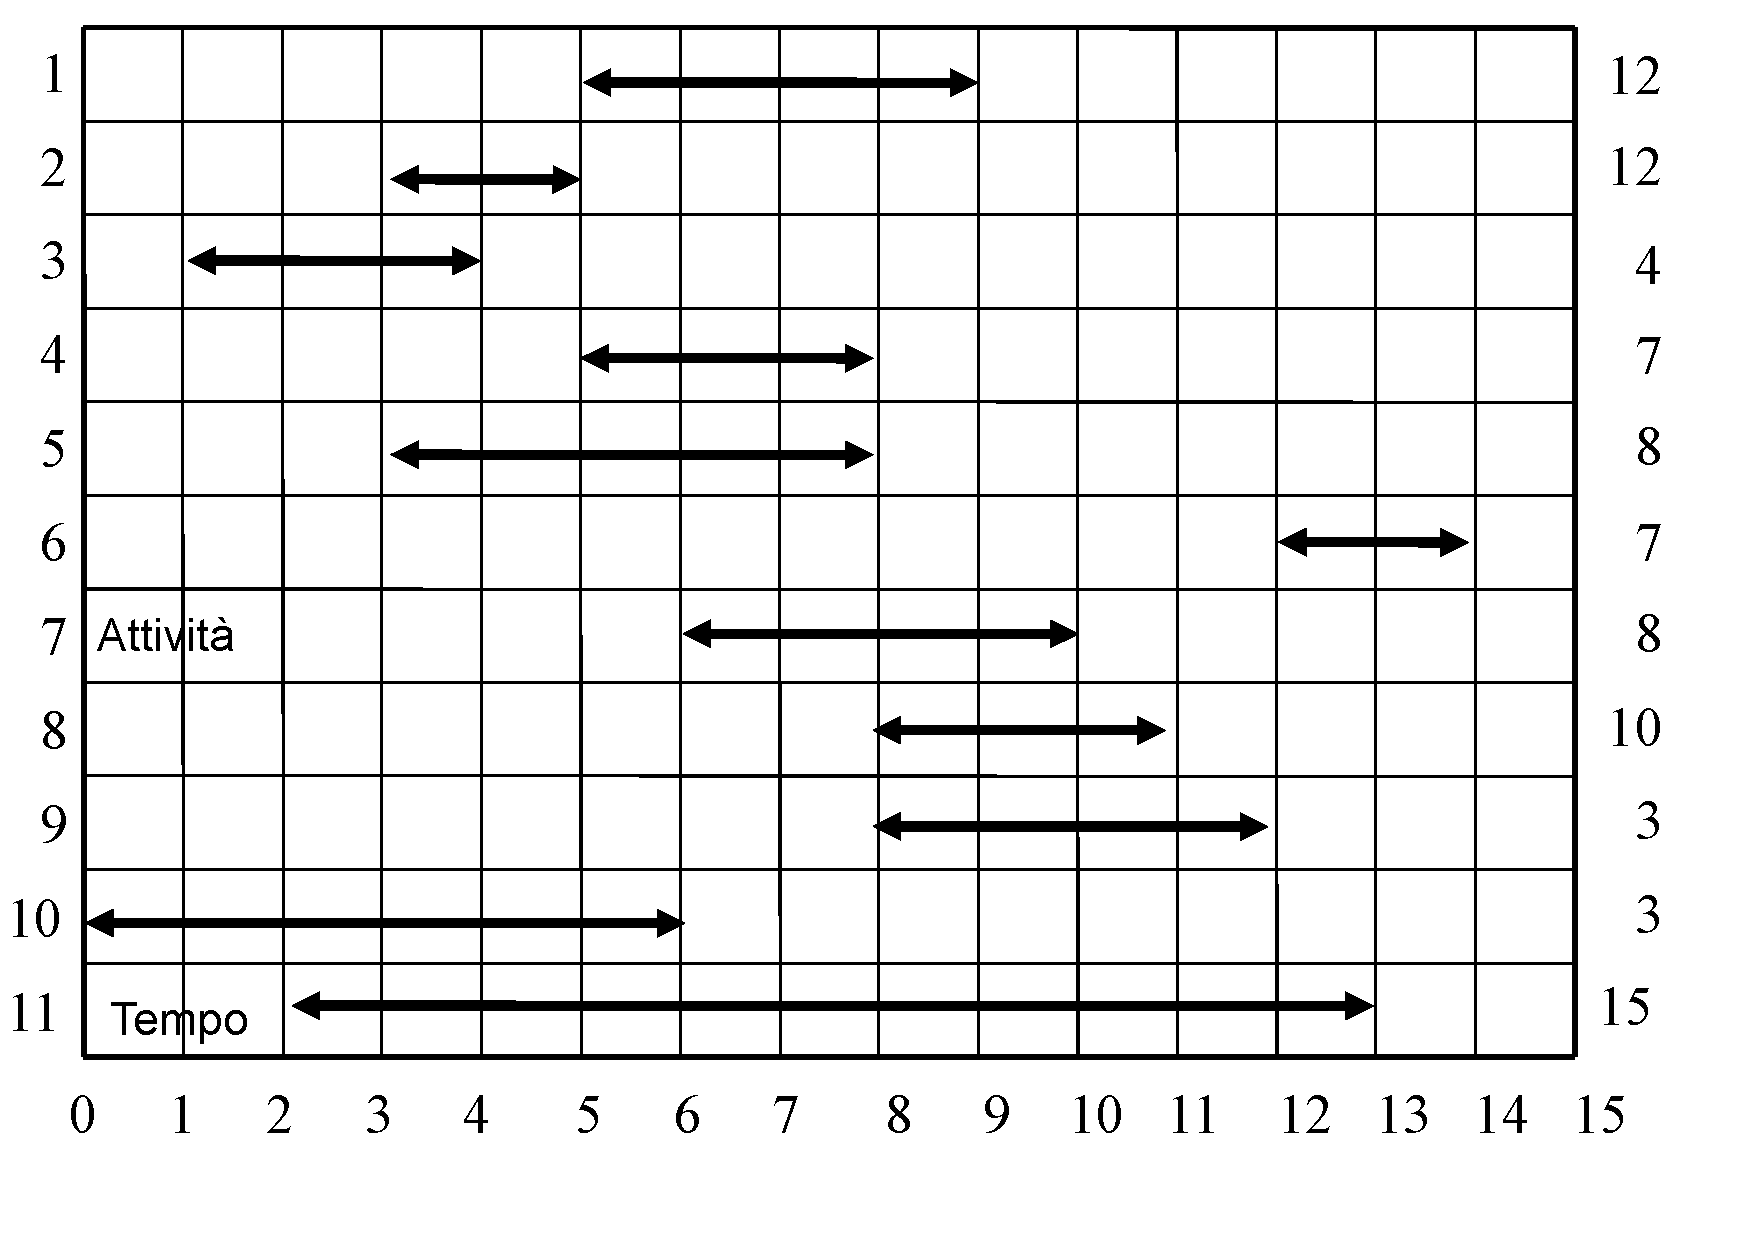
\includegraphics[width=0.95\textwidth,page=1]{intervalli-esempio.pdf}
\end{center}

\end{frame}

%-------------------------------------------------------------------------
\begin{frame}{Esempio -- Ordinato per estremi di fine non-decrescenti}

\vspace{-12pt}
\begin{center}
\includegraphics[width=0.95\textwidth,page=2]{intervalli-esempio.pdf}
\end{center}

\end{frame}

%-------------------------------------------------------------------------
\begin{frame}{Esempio -- Ordinato per estremi di fine non-decrescenti}

\vspace{-12pt}
\begin{center}
\includegraphics[width=0.95\textwidth,page=3]{intervalli-esempio.pdf}
\end{center}

\end{frame}

%-------------------------------------------------------------------------
\begin{frame}{Pre-elaborazione}

\vspace{-9pt}
\BB{
Per usare PD, è necessario effettuare una pre-elaborazione: ordinare gli intervalli per estremi finali non decrescenti
  \[
     b_1 \leq b_2 \leq \ldots \leq b_n
  \]
}

\begin{myboxtitle}[Profitto massimo (Versione 1)]
$DP[i]$ contiene il profitto massimo ottenibile con i primi $i$ intervalli
\small
\[
  DP[i] = \begin{cases}
    0 & i = 0 \\
    \max (DP[i-1], \max \{ DP[j]+w_i : j < i \wedge b_j \leq a_i \} ) & i > 0
  \end{cases}
\]
\end{myboxtitle}

\begin{myboxtitle}[Costo computazionale?]
\pause 
$O(n^2)$
\end{myboxtitle}

\end{frame}

%-------------------------------------------------------------------------
\begin{frame}{Pre-elaborazione}

\vspace{-9pt}
\BB{
Una seconda possibile pre-elaborazione consiste nel pre-calcolare il \alert{predecessore} \alert{$\mathit{pred}_i = j$} di $i$, dove:
\BIL
\item $j<i$ è il massimo indice tale che $b_j \leq a_i$
\item se non esiste tale indice, $\mathit{pred}_i=0$.
\EIL
}

\begin{center}
\IG{0.6}{predecessore.pdf}
\end{center}

\begin{myboxtitle}[Profitto massimo (Versione 2)]
\[
  DP[i] = \begin{cases}
    0 & i = 0 \\
    \max (DP[i-1], DP[\mathit{pred}_i] + w_i) & i > 0
  \end{cases}
\]
\end{myboxtitle}

\end{frame}

%-------------------------------------------------------------------------
\begin{frame}{Pre-elaborazione - calcolo predecessori}

\vspace{-6pt}
\begin{Procedure}
\caption[A]{$\INTEGER[\,]$ \textsf{computePredecessor($\INTEGER[\,]\ a$, $\INTEGER[\,]\ a$, \INTEGER $n$)}}    
$\INTARRAY\ \mathit{pred} = \NEW\ \INTEGER[0 \ldots n]$\;
$\mathit{pred}[0] = 0$\;
\For{$i = 1$ \TO $n$}{
  $j = i - 1$\;
  \While{$j > 0$ \AND\ $b[j] > a[i]$}{
    $j = j-1$\;
  }
  $\mathit{pred}[i] = j$\;
}
\Return $\mathit{pred}$\;
\end{Procedure}

\vspace{-6pt}
\begin{columns}[T]
\column{0.65\textwidth}
\BB{Quanto costa pre-calcolare i predecessori?}
\pause
\column{0.25\textwidth}
\bigskip\smallskip
$O(n^2)$
\end{columns}

\begin{columns}[T]
\column{0.65\textwidth}
\BB{Si può fare meglio di così?}
\pause
\column{0.25\textwidth}
\bigskip\smallskip
Sì! $O(n \log n)$
\end{columns}

\end{frame}

\begin{frame}{Alcune note}
    
\BIL
\item Gli intervalli vanno ordinati per tempo non decrescente di fine
\item Eventuali intervalli con lo stesso tempo di fine possono essere ordinati in qualunque modo
\item Questo perché ogni valore $DP[i]$ rappresenta il massimo profitto ottenibile con i primi $i$ intervalli
\item \EE quindi possibile escludere l'intervallo $i$-esimo se sceglierne uno precedente $j$ (ma con lo stesso tempo di fine $b[i]=b[j]$) ha un valore $DP[j]$ più alto
\EIL

\end{frame}


%-------------------------------------------------------------------------
\begin{frame}[shrink=10]{Versione completa}

\vspace{-12pt}
\begin{Procedure}
\caption[A]{\Set\ \maxinterval($\INTARRAY\ a,\ \INTARRAY\ b,\ \INTARRAY w$, \INTEGER $n$)}	

\{ ordina gli intervalli per estremi di fine crescenti \}\;
$\INTARRAY\ pred = \textsf{computePredecessor}(a,b,n)$\;
$\INTARRAY\ DP = \NEW\ \INTEGER[0 \mldots n]$\;
$DP[0] = 0$\;
\For{$i = 1$ \TO\ $n$}
{
  $DP[i] = \MAX(DP[i-1], w[i] + DP[\mathit{pred}[i]])$\;
}
$i = n$\;
$\Set\ S = \setconstructor()$\;
\While{$i>0$}
{
  \eIf{$DP[i-1]> w[i] + DP[\mathit{pred}[i]]$}{
    $i = i-1$\;
  }{
    $S.\setinsert(i)$\;
    $i = \mathit{pred}[i]$\;
  }
}
\Return $S$\;
\end{Procedure}

\end{frame}

%-------------------------------------------------------------------------
\begin{frame}{Costo computazionale}

\vspace{-9pt}
\begin{myboxtitle}[Costo computazionale]
\BIL
\item Ordinamento intervalli: \alert{$O(n \log n)$}
\item Calcolo predecessori: \alert{$O(n \log n)$}
\item Riempimento tabella $DP$: \alert{$O(n)$}
\item Ricostruzione soluzione: \alert{$O(n)$}
\item Algoritmo completo: \alert{$O(n \log n)$}
\EIL
\end{myboxtitle}

\begin{myboxtitle}[Esercizio]
Scrivere una funzione di calcolo predecessori in tempo $O(n \log n)$
\end{myboxtitle}

\end{frame}

%-------------------------------------------------------------------------
\begin{frame}{Insieme indipendente di intervalli pesati -- Conclusioni}

\vspace{-6pt}
\begin{myboxtitle}[Take-home message -- prendi e porta a casa]
Talvolta, può essere necessario pre-processare l'input per poter applicare nella maniera più efficiente la programmazione dinamica
\end{myboxtitle}

\end{frame}

%-------------------------------------------------------------------------
\begin{frame}{Per concludere}

\vspace{-6pt}
\begin{myboxtitle}[Una lezione ancora più importante]
La programmazione dinamica non è la soluzione di tutti i vostri problemi. Esistono altre tecniche che possono fare "meglio di così". Inoltre, è possibile che soluzioni ad-hoc possano essere migliori
\end{myboxtitle}

\begin{myboxtitle}[Esempi]
\BI
\item \alert{Moltiplicazione di matrici}: esiste soluzione $O(n \log n)$
\item \alert{Longest common subsequence}: può essere risolto in tempo $O(mn/\log n)$ (con alfabeto limitato)
\item \alert{Four Russians algorithm}: tecnica generale che può essere applicata a vari problemi su matrice con alfabeto limitato $O(n^2/\log n)$
\BI
\item Edit distance
\item Transitive closure, ...
\EI
\EI
\end{myboxtitle}

\end{frame}

%-------------------------------------------------------------------------
\begin{frame}{Approccio generale}

\vspace{-6pt}
\IG{1.0}{progrdyn.pdf}

\end{frame}

%-------------------------------------------------------------------------
\begin{frame}{Riassunto: programmazione dinamica / memoization}

\vspace{-6pt}
\begin{myboxtitle}[Fasi]
\BIL 
\item Caratterizzare la \alert{struttura} di una soluzione ottima
\item Dimostrare che la soluzione gode di \alert{sottostruttura ottima}
\item Definire ricorsivamente il \alert{valore} di una soluzione ottima
\item Calcolare il \alert{valore} di una soluzione ottima "bottom-up" (prog. dinamica) / "top-down" (memoization)
\item \alert{Ricostruzione} di una soluzione ottima 
\EIL
\end{myboxtitle}

\end{frame}

\end{document}


